To provide a comprehensive and representative view, the tests are structured into five subsections, each corresponding to a different Ethernet frame size. 
Four of the selected sizes -- 64 bytes, 512 bytes, 1280 bytes, and 1518 bytes -- are recommended by RFC~2544~\cite{rfc2544} 
covering both edge cases and practically relevant intermediate values. 
The fifth size, 889 bytes, was chosen based on real-world traffic analysis by Jurkiewicz et al.~\cite{JURKIEWICZ202115}, who identified it as the average frame size observed in modern network environment.
This selection covers the full range of standard Ethernet frame sizes, from the minimum to the maximum non-jumbo frames, 
while also including a statistically representative average.

All tests were conducted at four different transmission speeds -- 1, 10, 25, and 40 Gbit/s -- to evaluate the behavior of each configuration under varying network loads.  
These transmission rates reflect standard Ethernet link speeds as defined in IEEE~802.3~\cite{802.3}.

All traffic was generated using TRex with the profile included in Appendix~\ref{appendix:trex-profile},
which ensures that each packet carries a varying source IP address to simulate multiple concurrent clients, while maintaining a single destination IP per direction.
In all forwarding scenarios, a /24 source IP pool was used, while a /16 pool was employed in NAT scenarios to simulate a higher number of concurrent clients.
Since the aim of this thesis is to evaluate the VPP architecture rather than specific features (e.g., routing table lookup or hashing mechanisms),
the routing table of the DUT contains only two active forwarding entries corresponding to the test routes,
along with two administrative entries used for management purposes.

The DUT is configured with the VPP stack and tested under three levels of parallelism: using 1, 4, and 10 worker threads, plus a single main thread in all configurations.
The worker threads are pinned to the NUMA node closest to the NICs to minimize memory access latency.
The number of RX/TX queues is aligned with the number of active worker threads in each configuration to ensure balanced packet distribution and optimal resource utilization.
In the tables, the number of worker threads is denoted as VPP-X, where X indicates the number of worker threads used.

To provide a baseline for comparison, all scenarios are also executed using the standard Linux kernel networking stack.
It is configured with routing and interface parameters equivalent to the VPP setup, utilizing all 10 CPU cores on the NUMA node closest to the NICs.
Affinities are set evenly across the cores.
This allows for a direct comparison between VPP and traditional kernel-based forwarding in terms of performance and energy efficiency.
All CPU cores used for testing (including VPP scenarios) are set to performance mode, as is standard practice in network workloads.

In order to cover common real-world deployment scenarios, three traffic patterns were evaluated: one-way forwarding, bi-directional (both-way) forwarding, and NAT with forwarding.
These scenarios represent typical use cases encountered in small to medium-sized ISP or enterprise environments, where Linux or VPP may be deployed as the primary software-based router.
NAT is a commonly used feature in smaller ISP deployments. As it is a computationally intensive operation, the key question in this context is how it affects overall performance.

\subsection{One-way forwarding}

These tests were conducted in a one-way configuration, as suggested by \\RFC~2544~\cite{rfc2544}.
Such setup can represent asymmetric traffic patterns commonly found in real-world scenarios -- for example, downstream-heavy services like web servers or video streaming platforms.
It can also emulate high-load conditions similar to those observed during denial-of-service (DoS) attacks, where a large volume of traffic targets a single destination. 

%----------------------------------
\subsubsection{1 Gbps Test Results}

As can be seen from the results presented in Table~\ref{tab:one-way-1}, all configurations were able to successfully transmit all data in this low-traffic scenario.
The VPP-1 configuration performed best across all metrics. Even though this was the least demanding test scenario, the Linux stack still consumed more power than VPP-1.
In terms of latency, the Linux configuration outperformed both VPP-4 and VPP-10 at frame sizes of 1280B and 1518B.
However, latency in the Linux setup increased when switching from 1280B to 1518B frames, which can likely be attributed to internal kernel memory copying and buffer processing.
In contrast, all VPP configurations either maintained or slightly reduced latency with increasing frame size, demonstrating better scalability.
Interestingly, the single-threaded VPP-1 configuration achieved the lowest latency among all VPP variants.
This can likely be attributed to the absence of L3 cache thrashing and the ability to process more packets in a single batch, which amortizes the per-packet processing cost -- unlike parallelized VPP, 
which must traverse the processing graph with fewer packets per vector.
In low-demand scenarios, multithreading may become a disadvantage rather than an advantage.

\begin{table}[h!]
\centering
\caption{Results of one-way 1~Gbit/s tests}
\begin{tabular}{|c|l|r|r|r|r|}
\hline
\textbf{} & \textbf{Config} & \textbf{Energy [Wh]} & \textbf{Pkt Loss [\%]} & \textbf{Avg Lat [$\mu$s]} & \textbf{Jitter [$\mu$s]} \\
\hline
\multirow{4}{*}{\rotatebox{90}{64B}}    & VPP-1  & 5.68 & 0.00 & 12.80  & 9.50  \\
                                        & VPP-4  & 6.46 & 0.00 & 27.45  & 13.55 \\
                                        & VPP-10 & 7.86 & 0.00 & 28.30  & 12.65 \\
                                        & Linux  & 6.78 & 0.00 & 108.05 & 97.25 \\
\hline
\multirow{4}{*}{\rotatebox{90}{512B}}   & VPP-1  & 5.69 & 0.00 & 12.10  & 11.70 \\
                                        & VPP-4  & 6.48 & 0.00 & 22.85  & 17.40 \\
                                        & VPP-10 & 7.91 & 0.00 & 23.80  & 17.35 \\
                                        & Linux  & 6.23 & 0.00 & 56.10  & 51.35 \\
\hline
\multirow{4}{*}{\rotatebox{90}{889B}}   & VPP-1  & 5.76 & 0.00 & 10.30  & 8.40  \\
                                        & VPP-4  & 6.45 & 0.00 & 21.30  & 17.60 \\
                                        & VPP-10 & 7.85 & 0.00 & 20.95  & 16.30 \\
                                        & Linux  & 6.14 & 0.00 & 23.70  & 21.50 \\
\hline
\multirow{4}{*}{\rotatebox{90}{1280B}}  & VPP-1  & 5.72 & 0.00 & 8.10   & 5.80  \\
                                        & VPP-4  & 6.46 & 0.00 & 18.30  & 17.20 \\
                                        & VPP-10 & 7.84 & 0.00 & 18.80  & 15.95 \\
                                        & Linux  & 6.11 & 0.00 & 9.95   & 3.80  \\
\hline
\multirow{4}{*}{\rotatebox{90}{1518B}}  & VPP-1  & 5.66 & 0.00 & 7.20   & 5.50  \\
                                        & VPP-4  & 6.42 & 0.00 & 16.10  & 15.75 \\
                                        & VPP-10 & 7.84 & 0.00 & 17.65  & 17.35 \\
                                        & Linux  & 6.10 & 0.00 & 12.25  & 10.55 \\
\hline
\end{tabular}
\label{tab:one-way-1}
\end{table}

The energy efficiency of all configurations is shown in Fig.~\ref{fig:1g}. All VPP configurations maintained stable BPWh values, which is due to their busy-wait processing model.
The Linux stack becomes more efficient with increasing frame size, likely as a result of less frequent system calls.
As can be seen, even in the most favourable scenario, the Linux stack was not more energy-efficient than VPP-1, and when transmitting 64-byte frames, it was also less efficient than VPP-4.

\begin{figure}[!htbp]
    \centering
    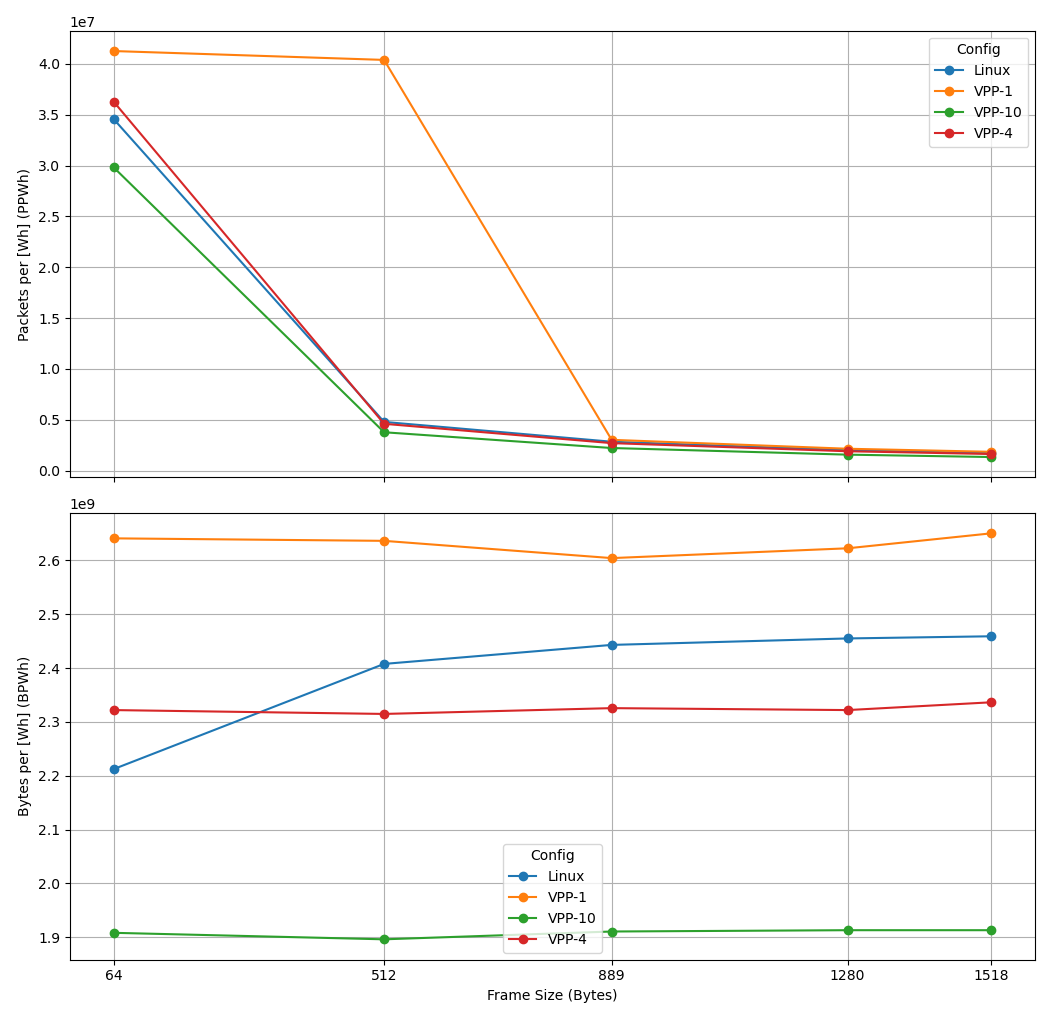
\includegraphics[width=\linewidth]{images/consumption-1g.png}
    \caption{Energy efficiency per delivered data in one-way 1\,Gbit/s}
    \label{fig:1g}
\end{figure}


%---------------------------------------------------------------------------------------------
%---------------------------------------------------------------------------------------------
%---------------------------------------------------------------------------------------------
\subsubsection{10 Gbps Test Results}

In the 10\,Gbit/s scenario, both VPP-1 and the Linux stack experienced significant difficulties delivering 64-byte frames, resulting in high packet loss and dramatically increased latency.
In contrast, all other configurations handled the traffic without loss, and latency generally decreased with increasing frame size.
A minor deviation from this trend was observed in the VPP-1 512-byte and VPP-4 64-byte frame tests, where latency temporarily increased with larger frame sizes before dropping again.
This suggests that VPP configurations may deliver optimal latency when operating near their forwarding capacity.
As observed before, VPP-1 consistently achieved the lowest latency among all VPP variants, except in the 64-byte test.
The Linux stack once again exhibited a latency increase when transitioning from 1280B to 1518B frames, as previously observed in the 1Gbit/s tests.
The detailed statistics are shown in Tab.~\ref{tab:one-way-10}

\begin{table}[h!]
\centering
\caption{Results of one-way 10~Gbit/s tests}
\begin{tabular}{|c|l|r|r|r|r|}
\hline
\textbf{} & \textbf{Config} & \textbf{Energy [Wh]} & \textbf{Pkt Loss [\%]} & \textbf{Avg Lat [$\mu$s]} & \textbf{Jitter [$\mu$s]} \\
\hline
\multirow{4}{*}{\rotatebox{90}{64B}}    & VPP-1  & 5.72 & 59.50 & 589.50  & 14.05  \\
                                        & VPP-4  & 6.56 & 0.02  & 20.60   & 6.00   \\
                                        & VPP-10 & 8.04 & 0.00  & 30.00   & 12.90  \\
                                        & Linux  & 7.35 & 80.97 & 3846.30 & 217.80 \\
\hline
\multirow{4}{*}{\rotatebox{90}{512B}}   & VPP-1  & 5.60 & 0.00  & 19.95   & 12.00  \\
                                        & VPP-4  & 6.48 & 0.00  & 28.20   & 14.50  \\
                                        & VPP-10 & 7.97 & 0.00  & 29.05   & 13.65  \\
                                        & Linux  & 6.85 & 0.00  & 129.40  & 99.35  \\
\hline
\multirow{4}{*}{\rotatebox{90}{889B}}   & VPP-1  & 5.62 & 0.00  & 23.40   & 14.95  \\
                                        & VPP-4  & 6.48 & 0.00  & 26.50   & 18.25  \\
                                        & VPP-10 & 7.95 & 0.00  & 26.95   & 17.55  \\
                                        & Linux  & 6.67 & 0.00  & 66.45   & 68.30  \\
\hline
\multirow{4}{*}{\rotatebox{90}{1280B}}  & VPP-1  & 5.58 & 0.00  & 22.80   & 17.05  \\
                                        & VPP-4  & 6.47 & 0.00  & 25.95   & 16.90  \\
                                        & VPP-10 & 7.98 & 0.00  & 26.80   & 16.60  \\
                                        & Linux  & 6.54 & 0.00  & 57.05   & 65.50  \\
\hline
\multirow{4}{*}{\rotatebox{90}{1518B}}  & VPP-1  & 5.57 & 0.00  & 20.45   & 14.95  \\
                                        & VPP-4  & 6.48 & 0.00  & 24.00   & 17.45  \\
                                        & VPP-10 & 7.97 & 0.00  & 25.40   & 17.70  \\
                                        & Linux  & 6.51 & 0.00  & 61.75   & 65.80  \\
\hline
\end{tabular}
\label{tab:one-way-10}
\end{table}

Figure~\ref{fig:10g} illustrates the energy efficiency of each configuration in this test.
The significant drop in performance for VPP-1 and Linux during the 64-byte frame test is attributed to high packet loss.
When all packets are successfully delivered, all VPP configurations maintain stable BPWh values, as observed in the previous test.
In contrast, the Linux stack showed a decline in performance across all frame sizes.

\begin{figure}[!htbp]
    \centering
    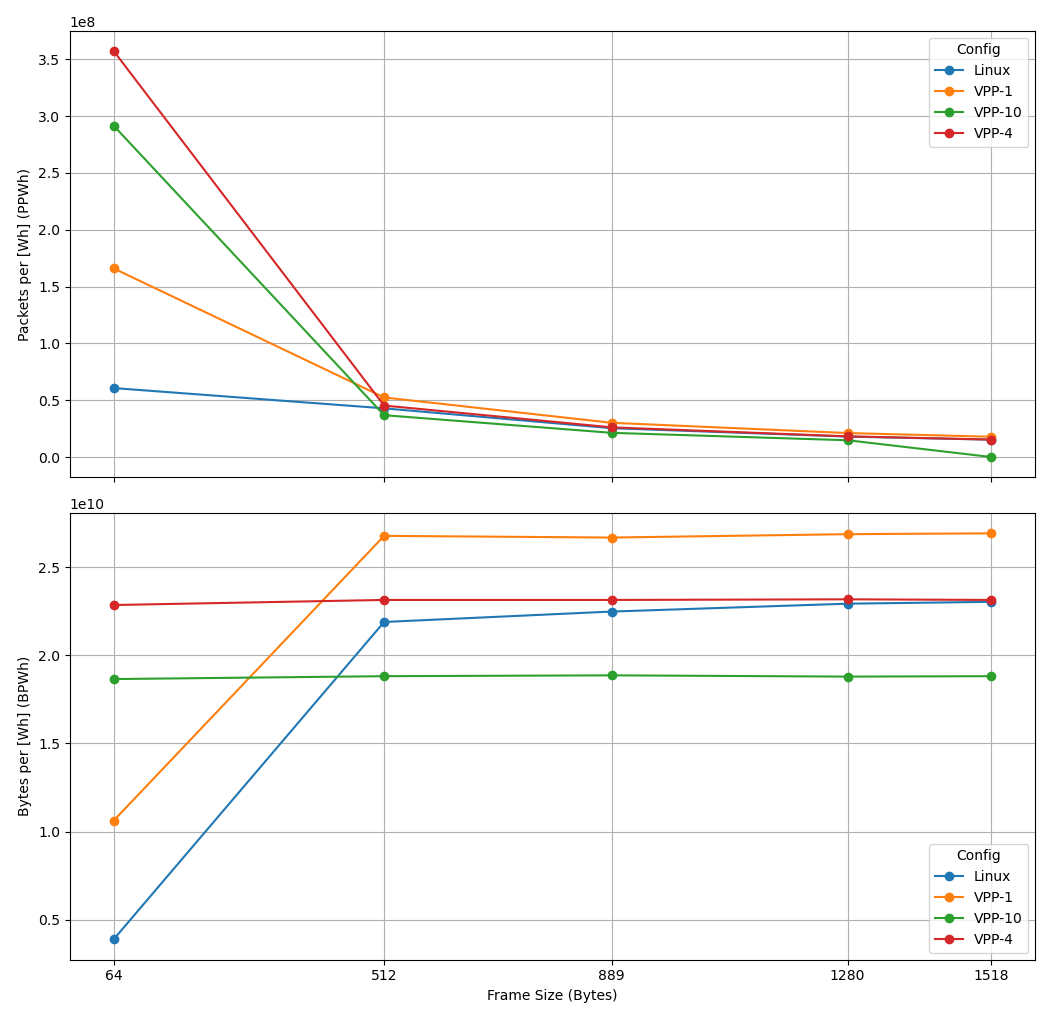
\includegraphics[width=\linewidth]{images/consumption-10g.png}
    \caption{Energy efficiency per delivered data in one-way 10\,Gbit/s}
    \label{fig:10g}
\end{figure}



%---------------------------------------------------------------------------------------------
%---------------------------------------------------------------------------------------------
%---------------------------------------------------------------------------------------------
\subsubsection{25 Gbps Test Results}

As shown in Table~\ref{tab:one-way-25}, none of the configurations were able to deliver all 64-byte frames, which naturally resulted in high latency in that test.
It can be observed that increasing the frame size beyond 889 bytes had no measurable impact on the performance of any VPP configuration -- the results remain comparable to the previous test.
In contrast, the Linux stack benefited from larger frames, and the increase in latency in prevoius test seen in the 1518-byte scenario compared to the 1280-byte scenario 
did not occur at this higher transmission rate.
An interesting observation is that when VPP drops packets, the ones that are not dropped tend to be delivered with significantly lower latency.

\begin{table}[h!]
\centering
\caption{Results of one-way 25~Gbit/s tests}
\begin{tabular}{|c|l|r|r|r|r|}
\hline
\textbf{} & \textbf{Config} & \textbf{Energy [Wh]} & \textbf{Pkt Loss [\%]} & \textbf{Avg Lat [$\mu$s]} & \textbf{Jitter [$\mu$s]} \\
\hline
\multirow{4}{*}{\rotatebox{90}{64B}}    & VPP-1  & 5.59 & 83.29 & 577.50   & 7.70   \\
                                        & VPP-4  & 6.56 & 49.00 & 198.85   & 7.65   \\
                                        & VPP-10 & 8.26 & 29.55 & 155.35   & 11.95  \\
                                        & Linux  & 7.43 & 92.71 & 5597.95  & 632.00 \\
\hline
\multirow{4}{*}{\rotatebox{90}{512B}}   & VPP-1  & 5.57 & 0.07  & 31.85    & 11.15  \\
                                        & VPP-4  & 6.43 & 0.00  & 29.55    & 13.75  \\
                                        & VPP-10 & 8.03 & 0.00  & 31.00    & 14.45  \\
                                        & Linux  & 7.57 & 47.97 & 7819.60  & 477.55 \\
\hline
\multirow{4}{*}{\rotatebox{90}{889B}}   & VPP-1  & 5.67 & 0.00  & 23.45    & 11.15  \\
                                        & VPP-4  & 6.39 & 0.00  & 30.50    & 15.50  \\
                                        & VPP-10 & 8.01 & 0.00  & 29.45    & 15.55  \\
                                        & Linux  & 7.42 & 0.87  & 166.05   & 111.15 \\
\hline
\multirow{4}{*}{\rotatebox{90}{1280B}}  & VPP-1  & 5.68 & 0.00  & 23.85    & 10.30  \\
                                        & VPP-4  & 6.48 & 0.00  & 31.15    & 15.40  \\
                                        & VPP-10 & 7.98 & 0.00  & 28.40    & 16.15  \\
                                        & Linux  & 7.10 & 0.00  & 146.90   & 126.20 \\
\hline
\multirow{4}{*}{\rotatebox{90}{1518B}}  & VPP-1  & 5.70 & 0.00  & 24.45    & 14.90  \\
                                        & VPP-4  & 6.46 & 0.00  & 30.60    & 15.80  \\
                                        & VPP-10 & 7.96 & 0.00  & 28.90    & 15.65  \\
                                        & Linux  & 7.00 & 0.00  & 130.00   & 105.30 \\
\hline
\end{tabular}
\label{tab:one-way-25}
\end{table}

Figure~\ref{fig:25g} illustrates the energy efficiency observed during the 25~Gbit/s test.
The drop in BPWh across all configurations in 64-byte frame test is primarily caused by high packet loss.
Compared to the previous test, the Linux stack performed significantly worse -- even at the largest frame size -- while all VPP configurations maintained stable BPWh values, 
except in the case of 64-byte frames.

\begin{figure}[!htbp]
    \centering
    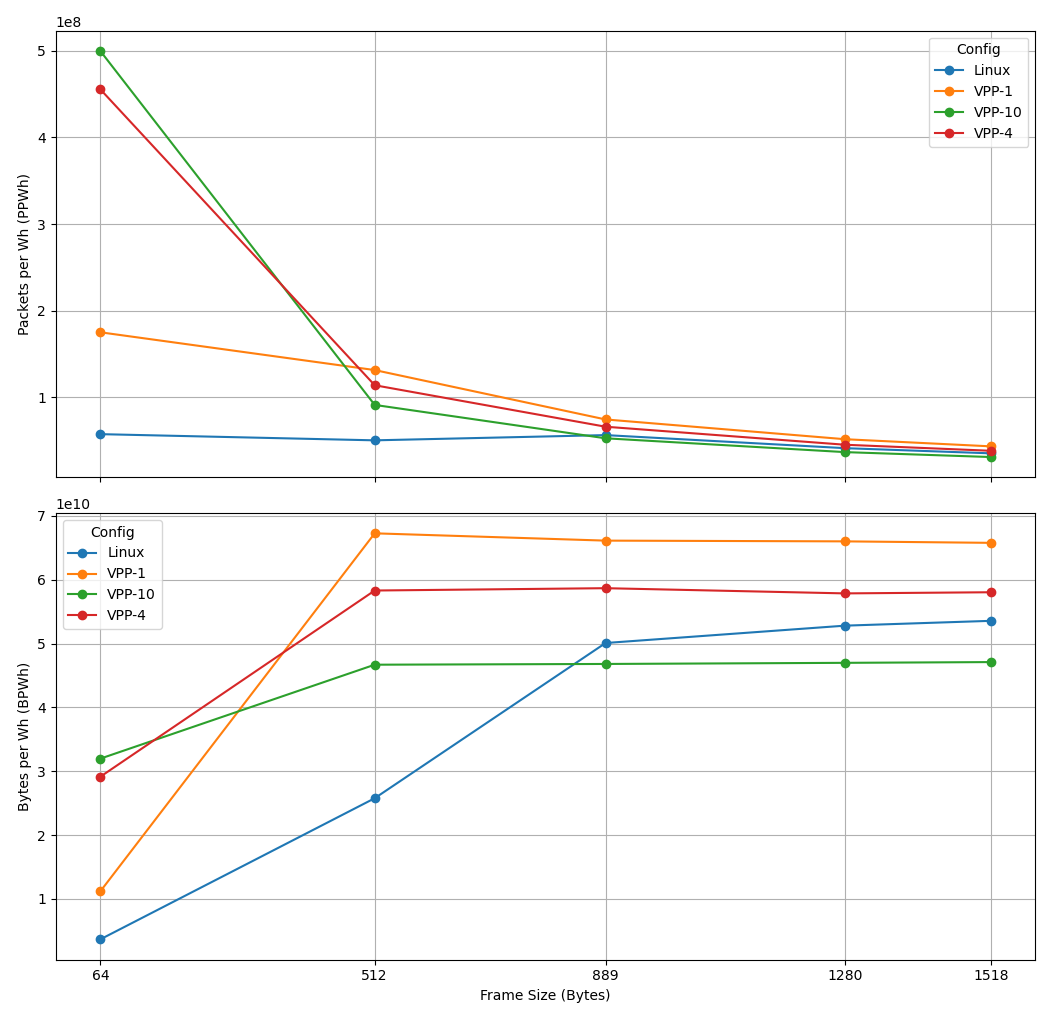
\includegraphics[width=\linewidth]{images/consumption-25g.png}
    \caption{Energy efficiency per delivered data in one-way 25\,Gbit/s}
    \label{fig:25g}
\end{figure}


%-----------------------------------
\subsubsection{40 Gbps Test Results}

As shown in Table~\ref{tab:one-way-40}, the 64-byte frame test resulted in even higher packet loss than in the previous test.
However, the latency statistics for VPP remained comparable to those observed earlier, despite the increased loss.
In this test, the Linux stack failed to deliver all data across all frame sizes, which again led to consistently high latency.
When no data were dropped, all VPP configurations performed similarly, maintaining low and stable latency.
These results clearly highlight the advantage of VPP over the Linux network stack under heavy traffic loads.
Notably, even the least resource-intensive VPP configuration (VPP-1) significantly outperformed the Linux stack in both latency and reliability, 
demonstrating VPP’s efficiency even with minimal parallelism.\looseness=1

\begin{table}[h!]
\centering
\caption{Results of one-way 40~Gbit/s tests}
\begin{tabular}{|c|l|r|r|r|r|}
\hline
\textbf{} & \textbf{Config} & \textbf{Energy [Wh]} & \textbf{Pkt Loss [\%]} & \textbf{Avg Lat [$\mu$s]} & \textbf{Jitter [$\mu$s]} \\
\hline
\multirow{4}{*}{\rotatebox{90}{64B}}    & VPP-1  & 5.60 & 89.53 & 576.00   & 6.50   \\
                                        & VPP-4  & 6.57 & 67.54 & 195.70   & 6.57   \\
                                        & VPP-10 & 8.12 & 54.38 & 152.05   & 9.20   \\
                                        & Linux  & 7.34 & 95.43 & 5629.05  & 550.30 \\
\hline
\multirow{4}{*}{\rotatebox{90}{512B}}   & VPP-1  & 5.82 & 35.26 & 292.45   & 122.15 \\
                                        & VPP-4  & 6.56 & 0.00  & 28.80    & 9.90   \\
                                        & VPP-10 & 8.00 & 0.00  & 35.45    & 14.35  \\
                                        & Linux  & 7.56 & 69.84 & 6621.50  & 892.35 \\
\hline
\multirow{4}{*}{\rotatebox{90}{889B}}   & VPP-1  & 5.77 & 3.85  & 203.05   & 25.20  \\
                                        & VPP-4  & 6.54 & 0.00  & 32.55    & 13.75  \\
                                        & VPP-10 & 8.00 & 0.00  & 33.60    & 18.50  \\
                                        & Linux  & 7.63 & 49.85 & 7222.80  & 315.40 \\
\hline
\multirow{4}{*}{\rotatebox{90}{1280B}}  & VPP-1  & 5.79 & 0.00  & 32.50    & 14.65  \\
                                        & VPP-4  & 6.40 & 0.00  & 33.95    & 14.35  \\
                                        & VPP-10 & 8.02 & 0.00  & 32.15    & 16.85  \\
                                        & Linux  & 7.59 & 6.25  & 2830.95  & 104.10 \\
\hline
\multirow{4}{*}{\rotatebox{90}{1518B}}  & VPP-1  & 5.83 & 0.00  & 30.35    & 15.75  \\
                                        & VPP-4  & 6.43 & 0.00  & 34.20    & 14.75  \\
                                        & VPP-10 & 8.02 & 0.00  & 33.30    & 14.80  \\
                                        & Linux  & 7.36 & 0.08  & 195.05   & 122.05 \\
\hline
\end{tabular}
\label{tab:one-way-40}
\end{table}

The energy efficiency graph shown in Fig.~\ref{fig:40g} illustrates that VPP maintained stable BPWh values when no packets were dropped, 
while the Linux stack again exhibited even lower energy efficiency per delivered data.
This result confirms and completes the trend observed in the previous tests.


\begin{figure}[!htbp]
    \centering
    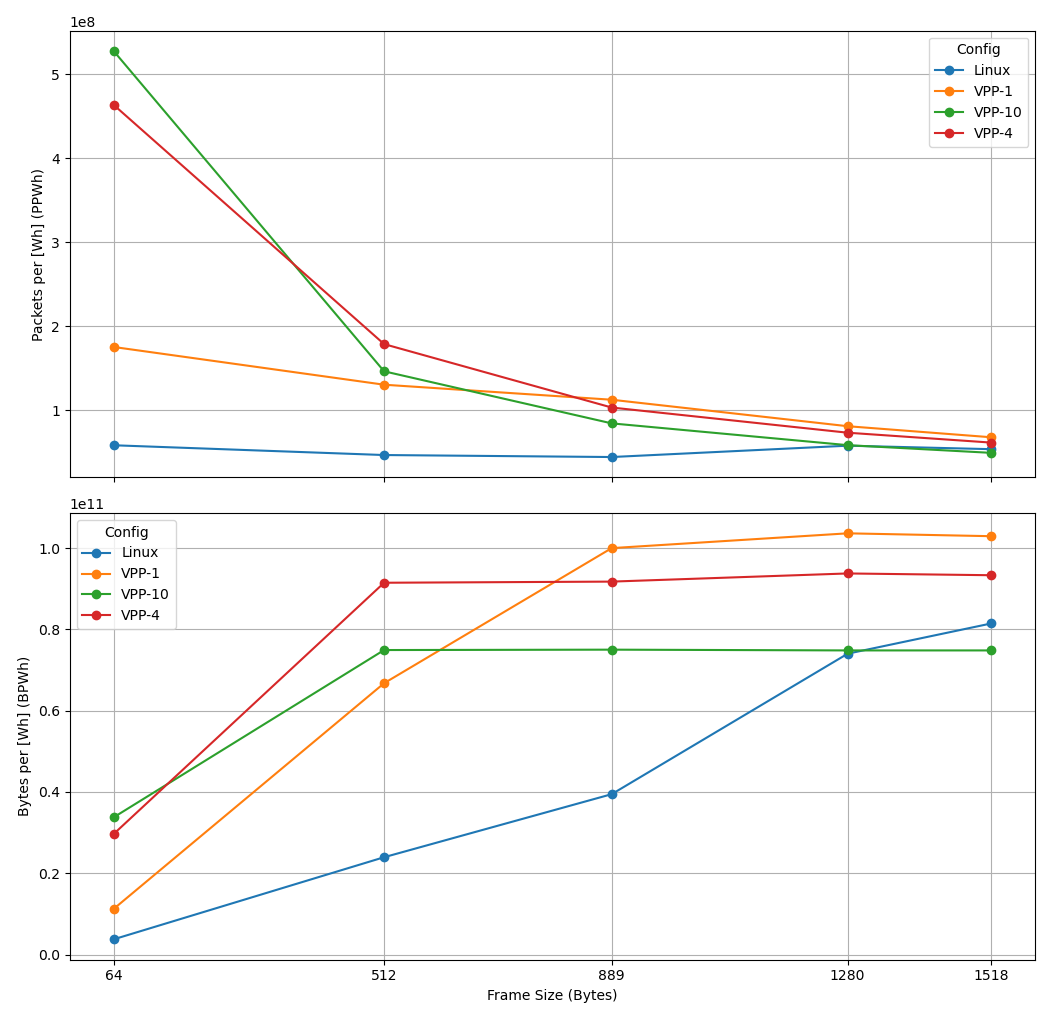
\includegraphics[width=\linewidth]{images/consumption-40g.png}
    \caption{Energy efficiency per delivered data in one-way 40\,Gbit/s}
    \label{fig:40g}
\end{figure}

